\chapter{User Interface Design \& Implementation}

\section{Updated Pages}

\subsection{Home Page}
\begin{figure}[H]
\centering
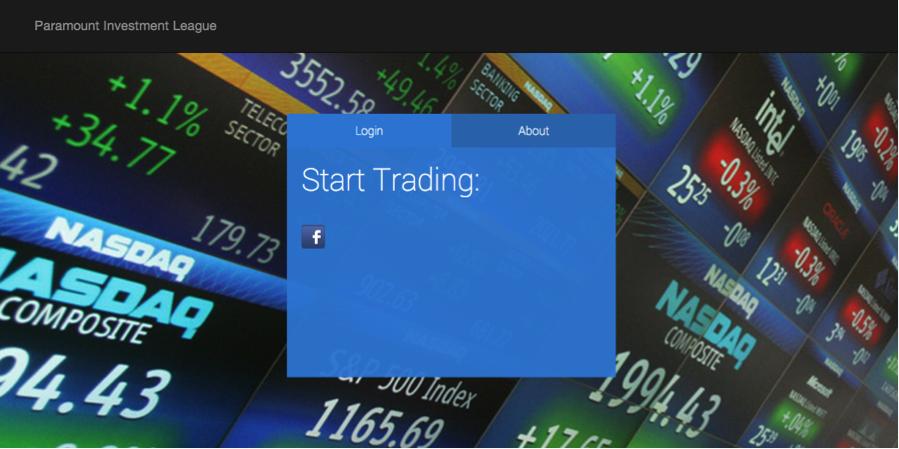
\includegraphics[width=5.5in]{./img/ui/1.png}
\caption{When a user firsts visits our website, they will have the ability to register through Facebook. A visitor can also view the about tab of our website.}
\end{figure}

\subsection{About Page}
\begin{figure}[H]
\centering
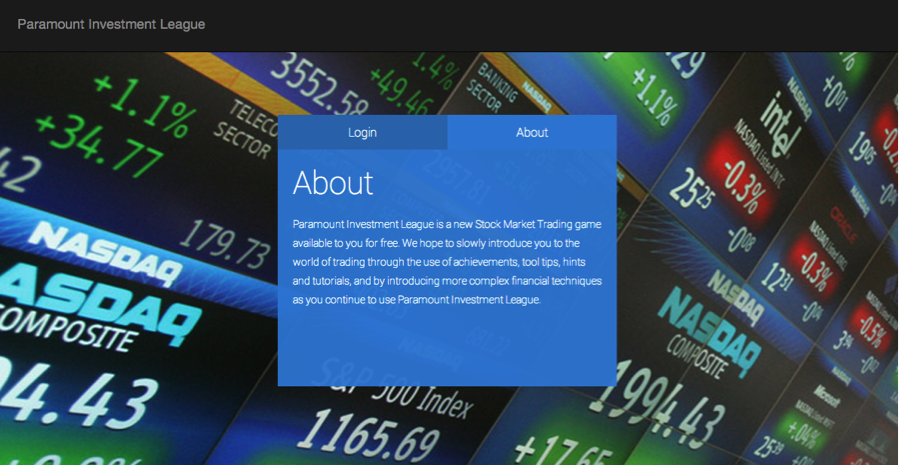
\includegraphics[width=5.5in]{./img/ui/2.png}
\caption{The figure above is our about page.}
\end{figure}

\subsection{Main Page}
\begin{figure}[H]
\centering
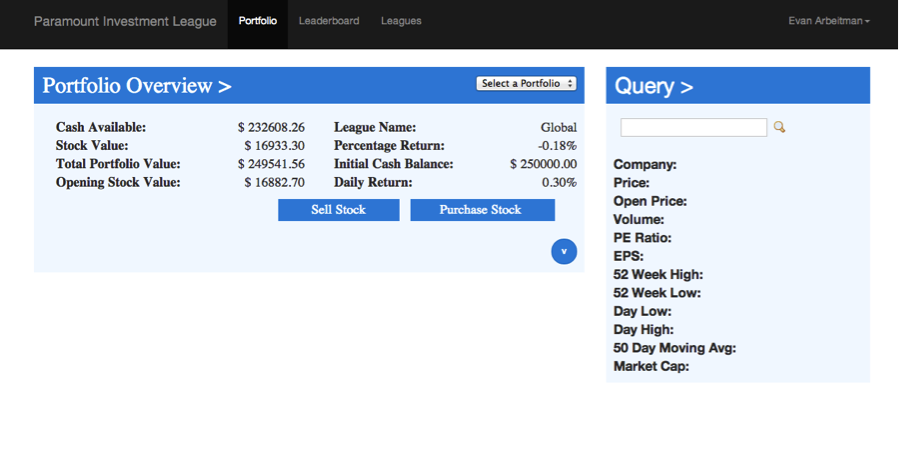
\includegraphics[width=5.5in]{./img/ui/3.png}
\caption{Once registered, the user will be brought to the main page. Here there are several things they can do.}
\end{figure}

\subsection{Buy/Sell Stock}
\begin{figure}[H]
\centering
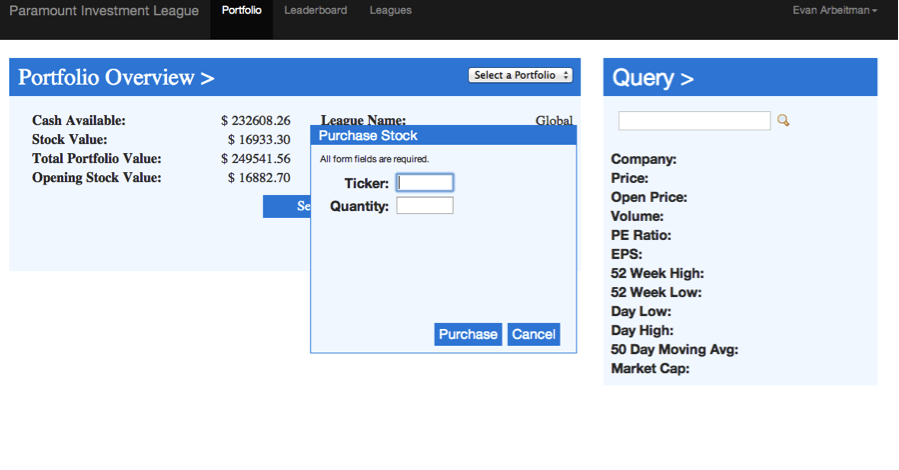
\includegraphics[width=5.5in]{./img/ui/4.png}
\caption{By pressing the purchase stock button on the main page, a small pop up window will appear and the user can enter the stock they want and the amount they want to purchase. The same pop up window will appear if the user clicks the sell stock option. This is shown in the figure above.}
\end{figure}

\subsection{View Leagues}
\begin{figure}[H]
\centering
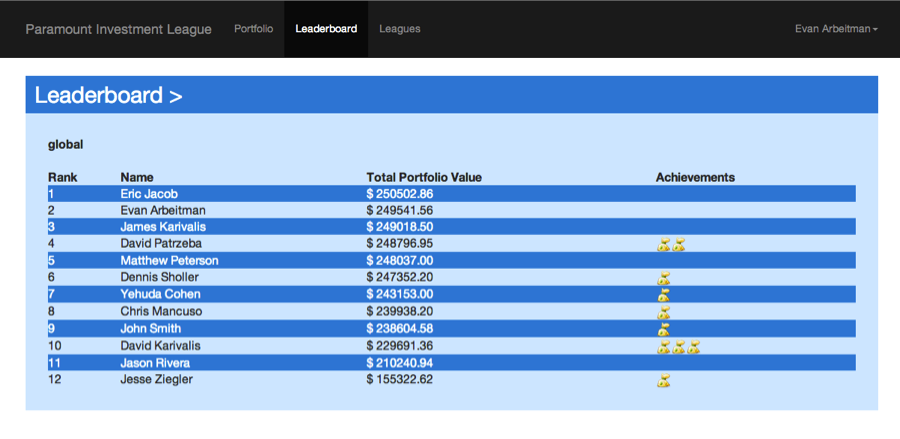
\includegraphics[width=5.5in]{./img/ui/5.png}
\caption{From the front page, the user can click the leaderboard tab and view all active members in a current league.}
\end{figure}

\subsection{Create a Public League}
\begin{figure}[H]
\centering
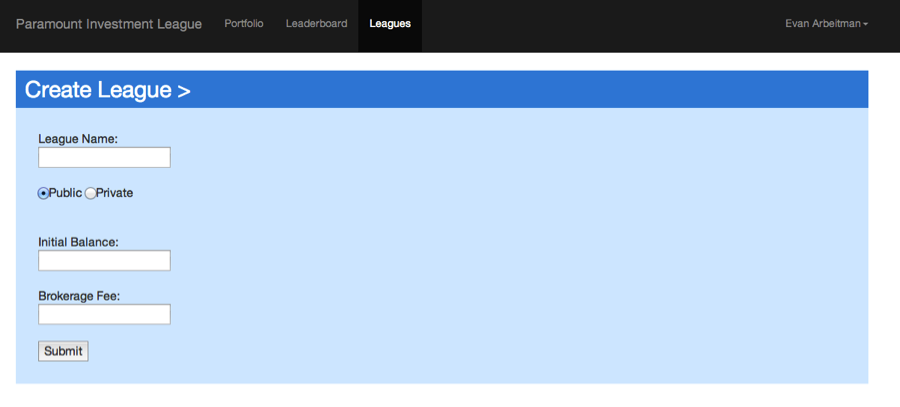
\includegraphics[width=5.5in]{./img/ui/6.png}
\caption{From the main page, the user can click the leagues tab and have the option to view, create, or join a league. In the figure above, the user who wants to create a league can choose to make the league public or private and set certain league rules.}
\end{figure}

\subsection{Create a Private League}
\begin{figure}[H]
\centering
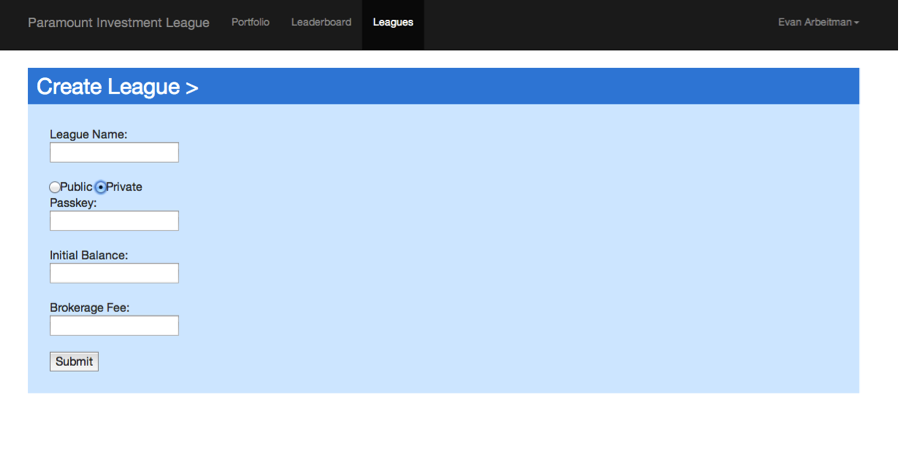
\includegraphics[width=5.5in]{./img/ui/7.png}
\caption{This is what the page will look like when they want to create a private league.}
\end{figure}

\subsection{View Leagues}
\begin{figure}[H]
\centering
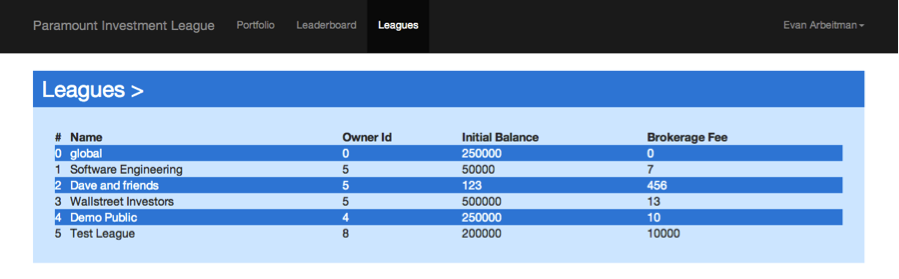
\includegraphics[width=5.5in]{./img/ui/8.png}
\caption{Users can view all relevant leagues as shown above.}
\end{figure}

\subsection{Query Stock}
\begin{figure}[H]
\centering
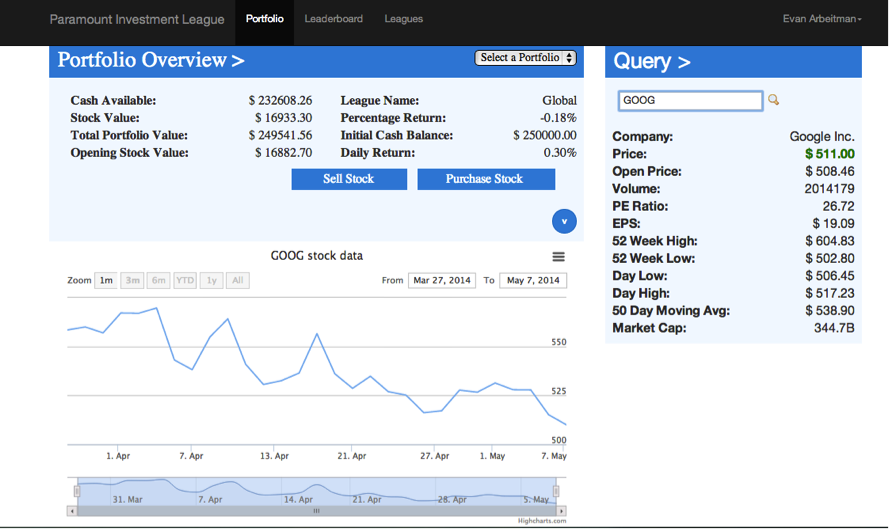
\includegraphics[width=5.5in]{./img/ui/9.png}
\caption{By querying a stock, user can see various features of that stock as well as graph displaying the value of stock over a time.}
\end{figure}


\section{Efficiency of the Views}

One thing that we need to concentrate on is ensuring that the website is fast
for all users no matter what kind of device or connection the end user is using.
For this reason, you will see a logical breakdown of the website which will
allow us to cache elements of the site on the client side that generally won't
change.  We do this be separating the header, ticker, and the content of a given
page.  Since the header and ticker are the same across the entire site, they
only need be loaded on the client a single time, and can be cached on the client
side for the duration of the visit or longer.\\

The content of each individual page is dynamic, but by harnessing technologies
like AJAX\cite{wiki:ajax} and Comet\cite{wiki:comt}, we are able to indicate to
the user that the page
is always reacting to their inputs without reloading the page.  This again
allows us to cache the resulting page on the client side, an perform updates
as needed with minimal delay.\\

To further assist with reducing the load on clients, we will be using
HTML\cite{wiki:html} and CSS\cite{wiki:css} to present our User Interface
relying very minimally on pictures.  Any picture that is displayed will be
resized to the maximum allowed size and contained in an appropriate web format.\\

Finally, as discussed much throughout these reports, our goal is to be able to
present our application across as many device as possible, including mobile,
tablet, and desktop.  We accomplish this by relying on the Twitter
Bootstrap\cite{wiki:boot} CSS framework to help facilitate creating a responsive
website.\\

Of course this all comes with a trade off, that is we won't support older
browsers incapable of displaying and parsing HTML5/CSS3/JS or aren't web
compliant with modern web standards.  This should have minimal impact however,
since most devices and users have a modern web browser, and those that don't
generally don't fall into our target audience.\\

\section{Home Page}

